%% LyX 2.0.7 created this file.  For more info, see http://www.lyx.org/.
%% Do not edit unless you really know what you are doing.
\documentclass{article}
\usepackage[margin=1in]{geometry}
\usepackage{graphicx}
\usepackage{bm}
\usepackage{bbm}
\usepackage{amsmath}
\usepackage{booktabs}
\usepackage{amsfonts}
%\usepackage{bbold}
\usepackage{sectsty}
\usepackage[compact]{titlesec}
\usepackage{color}
\usepackage[usenames,dvipsnames,svgnames,table]{xcolor}
\usepackage{mdframed}
%\usepackage{pgfornament}

% Paragraph settings
\setlength{\parindent}{0in}
\setlength{\parskip}{0.3cm}

% Title and section title spacing and formatting
\titlespacing{\chapter}{0pt}{*0}{*0}
\titlespacing{\section}{0pt}{*2.5}{*0}
\titlespacing{\subsection}{0pt}{*2}{*0}
%\allsectionsfont{\centering}
\sectionfont{\normalsize}
\subsectionfont{\normalsize \itshape}
\subsubsectionfont{\normalfont \itshape}

% new commands %
\newcommand{\pd}[2]{ \frac{\partial #1}{\partial #2} }
\newcommand{\comment}[1]{}
\newcommand{\p}[1]{ (#1_t)_{t \geq 0} }
\newcommand{\ch}[1]{ \{#1_t\}_{t \geq 0} }
\newcommand{\X}{\mathcal{X}}
\newcommand{\B}{\mathcal{B}}
%\newcommand{\proofbreak}{ \begin{center} \pgfornament[width = 10cm, color = black!60]{88} \end{center} }

\newcommand{\startboxblue}[1]{ \begin{mdframed}[linecolor=blue!40,linewidth=4pt, frametitle = {#1}, frametitlerule=true,
frametitlebackgroundcolor=gray!20, innertopmargin=\topskip, nobreak = true] }

\newcommand{\startboxgreen}[1]{ \begin{mdframed}[linecolor=Green!40,linewidth=4pt, frametitle = {#1}, frametitlerule=true,
frametitlebackgroundcolor=gray!20, innertopmargin=\topskip, nobreak = true] }

\newcommand{\startboxred}[1]{ \begin{mdframed}[linecolor=red!40,linewidth=4pt, frametitle = {#1}, frametitlerule=true,
frametitlebackgroundcolor=gray!20, innertopmargin=\topskip, nobreak = true] }

\newcommand{\finishbox}{\end{mdframed}}

\title{\Large \bfseries ABC-MCMC for Kamiltonian Sampler.}
\author{Sam Livingstone}
\date{\today}

\begin{document}
\maketitle


\section*{Likelihood-free Models}

Approximate Bayesian Computation is a method for inference in the
scenario where conditional on some parameter of interest $\theta$we
can easily simulate data $x\sim f(\cdot|\theta)$, but for which writing
the likelihood function $f$ is difficult/impossible. We generally
have some data $y$ which assume to be from the model, and we have
a prior $\pi_{0}(\theta)$. A simple ABC algorithm is to sample $\theta_{i}\sim\pi_{0}(\cdot)$
(or any other suitable distribution), simulate some data $x_i \sim f(\cdot|\theta_{i})$,
and `accept' $x_i$as a sample from the approximate posterior $\pi_{\epsilon}(\theta|y)$
if $d(y,x)\leq\epsilon$. This procedure can be formalised by defining
the approximate likelihood as
\begin{equation} \label{eqn:lik}
f_{\epsilon}(y|\theta)\propto\int g_{\epsilon}(y|x,\theta)f(x|\theta)dx,
\end{equation}


where $g_{\epsilon}(y|x,\theta)$ is some appropriate kernel that
gives more importance to points for which $d(y,x)$ is smaller. In
the simple case above $g_{\epsilon}(y|x,\theta) = \mathbbm{1}_{\{d(y,x) \leq \epsilon\}}$.
The ABC posterior is then found using $\pi_{\epsilon}(\theta|y)\propto f_{\epsilon}(y|\theta)\pi_{0}(\theta)$.
Often $g_{\epsilon}$is based on some low-dimensional summary statistics,
so `closeness' is defined through $d(S(y),S(x))$, which can have
both advantages and disadvantages.


\section*{Likelihood-free MCMC}

There are many different way to do ABC, and clearly not all involve
Markov chain Monte Carlo. But if the posterior
doesn't look much like the prior, and $\theta$ is more than three
or four dimensional, that it is usually a sensible option. Since the likelihood
is intractable typically algorithms are considered for which an approximation
to either the likelihood, the ABC posterior or in fact something else
are used either in constructing proposals, defining Metropolis-Hastings
acceptance rates, or both. I focus here on samplers which target $\pi_{\epsilon}(\theta|y)$
directly.


\subsection*{Pseudo-marginal Metropolis-Hastings}

Here proposals $\theta'\sim Q(\theta,\cdot)$ are accepted according
to the ratio
\begin{equation} \label{eqn:ratio}
\tilde{\alpha}(\theta,\theta')=\frac{\tilde{\pi}_{\epsilon}(\theta'|y)q(\theta|\theta')}{\tilde{\pi}_{\epsilon}(\theta|y)q(\theta'|\theta)},
\end{equation}


where $\tilde{\pi}_{\epsilon}(\theta|y)=\pi_{0}(\theta)\tilde{g}_{\epsilon}(y|\theta),$
and
\[
\tilde{g}_{\epsilon}(y|\theta)=\frac{1}{n}\sum_{i}g_{\epsilon}(y|x_{i},\theta), ~~ x_i \sim f(\cdot|\theta_i)
\]
is a simple Monte Carlo estimator for the intractable likelihood (\ref{eqn:lik}). Since
it is easy to simulate from $f$ then this is typically easy to compute.
As with other general pseudo-marginal schemes, it is crucial that
if $\theta'$ is accepted, the same estimate for $\tilde{\pi}(\theta'|y)$
is used on the denominator of the Hastings ratio in future iterations
until the next proposal is accepted for the scheme to produce a Markov
chain with limiting distribution $\pi_{\epsilon}(\cdot)$.


\subsection*{Monte Carlo within Metropolis}

A typical problem that with pseudo-marginal schemes is `sticking'.  If an estimate $\tilde{\pi}(\theta'|y)$ for a proposal $\theta'$ is surprisingly large, the proposal is likely to be accepted.  Keeping the same estimate on the denominator of the Hastings ratio when comparing to future proposals will mean that the acceptance ratio will be `artificially' small for these, meaning the chain can get stuck at this point.  To overcome this, a different option is to recompute the likelihood estimates in both the numerator and the denominator of (\ref{eqn:ratio}) at each iteration.  Although this strategy can result in faster mixing, it means that the Markov chain no longer has $\pi_\epsilon(\cdot)$ as its limiting distribution.  However, recent work \cite{roberts} suggests that this isn't such a problem.  If the original sampler is geometrically ergodic, typically the MCWM sampler will target a distribution which is `close' to $\pi_\epsilon(\cdot)$, so the slight bias trade off for improved mixing seems reasonable, especially as the ABC posterior $\pi_\epsilon(\cdot)$ is biased to begin with.

\subsection*{Synthetic Likelihood Metropolis-Hastings}

The idea here is to draw $n$ samples $x_i \sim f(\cdot|\theta_i)$, and fit a Gaussian approximation to $f$, producing estimates $\hat{\mu}$ and $\hat{\Sigma}$ for the mean and covariance using $\{x_i\}_{i = 1}^n$.  If the error functon $g_\epsilon$ is also chosen to be a Gaussian (with mean $y$ and variance $\epsilon$), then the marginal likelihood $f_\epsilon(y|\theta)$ can be approximated as
\[
y|\theta \sim \mathcal{N} \left( \hat{\mu},\hat{\Sigma} + \epsilon^2 I \right)
\]
So essentially the likelihood is being approximated by a Gaussian $f_G$, producing a synthetic posterior $\pi_s(\cdot)$ which is then used in the accept-reject step.  Clearly some approximation error is introduced by the Gaussian likelihood approximation step, but as shown in \cite{wood}, it can be a reasonable choice for some models.

\subsection*{Hamiltonian ABC}

Introduced in \cite{welling}, here the synthetic likelihood formulation is used to construct a proposal, with the accept-reject step removed altogether.  Hamiltonian dynamics use the gradient $\nabla\log\pi(\theta)$ to suggest candidate values for the next state of a Markov chain which are far from the current point, thus increasing the chances that the chain mixes quickly.  Here the gradient of the log-likelihood is unavailable, so is approximated with that of a Gaussian (since the map $\theta \to (\mu, \Sigma)$ is not always clear this is done numerically, with some tricks applied to ensure the gradient is estimated efficiently), giving
\[
\nabla\log\pi(\theta) \approx \sum_{i=1}^n \nabla\log  f_G(y_i|\hat{\mu}, \hat{\Sigma}) + \nabla\log\pi_0(\theta).
\]
Since there is no accept-reject step, the synthetic posterior is also the target of this scheme (although there is also further bias introduced by discretisation error), but the introduction of gradient-based dynamics should improve mixing and hence efficiency of inferences compared to random-walk type schemes.

\subsection*{Other Methods}

Other ABC-MCMC methods exists, for example based on using empirical density approximations to the likelihood, or sampling on the augmented $(x,\theta)$ space.  See \cite{sisson} for more details here.

\section*{Two simple examples}

An almost trivial toy model should highlight the bias introduced by the Hamiltonian ABC sampler.  A very simple example which should prove the point is posterior inference for the mean parameter in a log-Normal model.  Specfically, the true model is
\begin{align*}
\mu &\sim \mathcal{N}(\mu_0, \tau_0), \\
y|\mu, \tau &\sim \log\mathcal{N}(\mu, \tau), \\
\end{align*}
where the precision $\tau$ and hyperparameters $\mu_0, \tau_0$ are known.  The model is in fact conjugate, giving a Gaussian posterior
\[
\mu | y \sim \mathcal{N} \left( \frac{\tau_0\mu_0 + \tau \sum_i \log x_i}{\tau_0 + n\tau}, \tau_0 + n\tau \right)
\]
If we introduce a Gaussian approximation to the likelihood, then the mean and precision of this approximation $f_G$ should be (empirical estimates for)
\[
\mu_G = e^{\mu + 1/2\tau}, ~~ \tau_G = 1/\text{Var}[Y_i] = \frac{e^{-2\mu - 1/\tau}}{e^{1/\tau} - 1},
\]
which will change dependent on the current value for $\mu$ in the chain.  The resulting synthetic posterior is no longer tractable, but since it's one dimensional we can approximate it numerically and compare to the truth.  Putting some numbers in, if $\mu_0 = 0$, $\tau_0 = 1/100$, $\epsilon = 0.1$ and $\tau = 1$ then the true and approximate posteriors for 100 data points generated using the truth $\mu = 2$ are shown below.
\begin{figure}[h]
\begin{center}
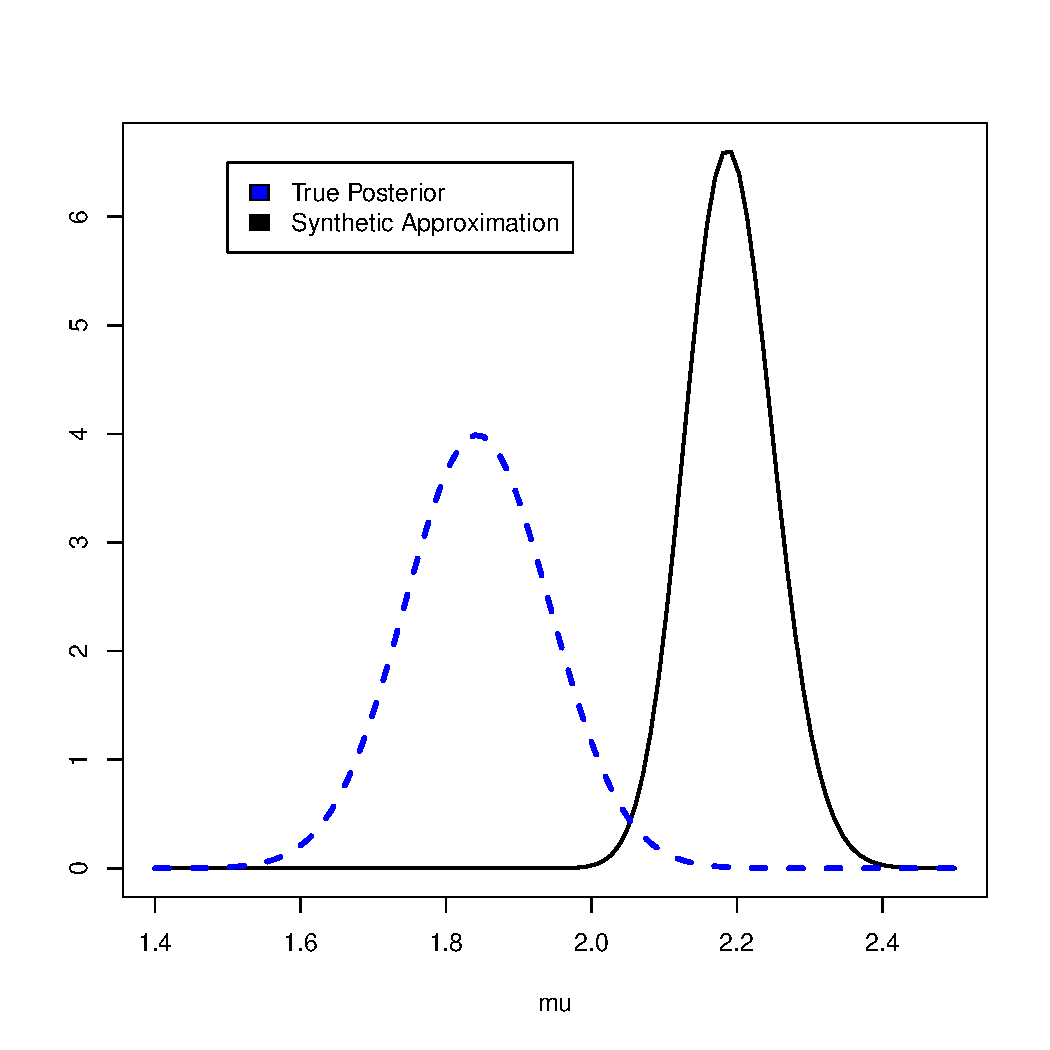
\includegraphics[width = 14cm]{LN_plot.pdf}
\end{center}
\end{figure}

The Kamiltonian sampler will, of course, target the true posterior.

This is essentially a proof of concept that a likelihood with some positive skew being approximated by a Gaussian should bias the posterior upwards.  A slightly more complex and multi-dimensional simulation example would be to take the likelihood as a multivariate skew-Normal distribution (e.g. \cite{kollo})
\[
f(y|\mu) = 2f_{N(\mu, \Sigma)}(y)\Phi( \langle\alpha, y \rangle),
\]
where $f_{N(\mu, \Sigma)}$ is a multivariate Gaussian density with chosen mean and covariance, $\alpha$ is a skewness vector (choose each $\alpha_i > 0$ for positive skew), and $\Phi$ is the standard $\mathcal{N}(0,1)$ CDF.  Generating some data with a reasonable size of $\alpha$ (there are R packages to simulate from this distribution) should mean that Gaussian likelihood approximations bias posterior inference for $\mu$.

\section*{Theory}

There is some work related to ABC-MCMC and approximate sampler that I am getting familiar with at the moment but I need more time to make something concrete out of this, so for now the introduction and example is what I have.

  \begin{thebibliography}{1}

  \bibitem{wood} Wood, Simon N. ``Statistical inference for noisy nonlinear ecological dynamic systems." \emph{Nature 466}, no. 7310 (2010): 1102-1104.

  \bibitem{sisson}  Sisson, Scott A., and Yanan Fan. ``Likelihood-Free MCMC." \emph{Handbook of MCMC Chapter 12} (2011): 313-333.

  \bibitem{turner} Turner, Brandon M. and Sederberg, Per B. ``A generalized, likelihood-free method for posterior estimation." \emph{Psychonomic Bulletin \& Review}, 21(2):227–250, 2014.
  
  \bibitem{roberts}  Medina-Aguayo, Felipe J., Anthony Lee, and Gareth O. Roberts. ``Stability of Noisy Metropolis-Hastings." \emph{arXiv preprint arXiv:1503.07066} (2015).
  
  \bibitem{welling} Meeds, Edward, Robert Leenders, and Max Welling. ``Hamiltonian ABC." \emph{arXiv preprint arXiv:1503.01916} (2015).
  
  \bibitem{kollo} Kollo, Tõnu, and J. Liivi. ``Skewed multivariate distributions." In \emph{Weekly Seminar in Statistics}. 2007.



  \end{thebibliography}

\end{document}
